\subsection{Scalability}
\vspace{-0.4cm}
\section{Experiments}
\vspace{-0.3cm}

\begin{figure*}[t]
\vspace{-0.4cm}
\centering
\begin{tabular}{|c|c|c|c|}
\hline
\multicolumn{2}{|c|}{\bf Topic Modeling} & {\bf Dictionary Learning} & {\bf MMND} \\
\hline
Convergence Plots & Scaling in \# Cores & Convergence Plots &  Convergence Plots \\
%\multicolumn{4}{|c|}{\bf Topic Modeling} \\
%\hline
%Convergence Plots & \# of Topics & \# of Processors & \# of Docs \\
\hline
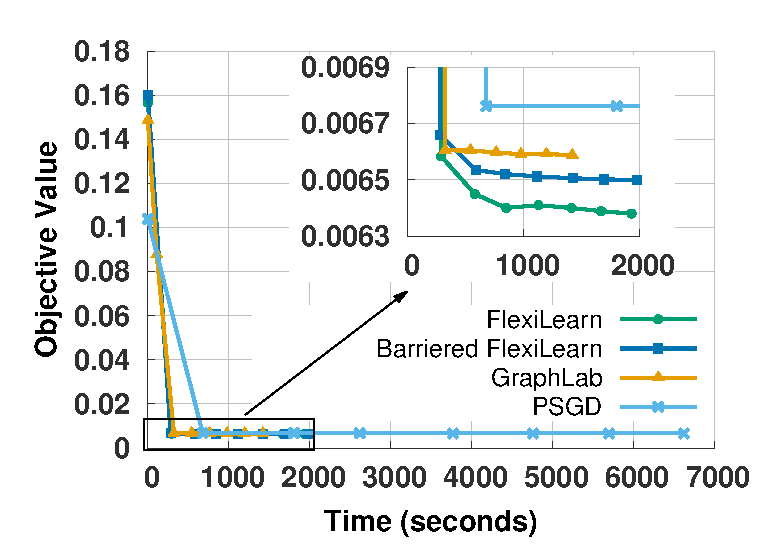
\includegraphics[width=0.23\textwidth]{fig2/lda_convergence.eps} 
& 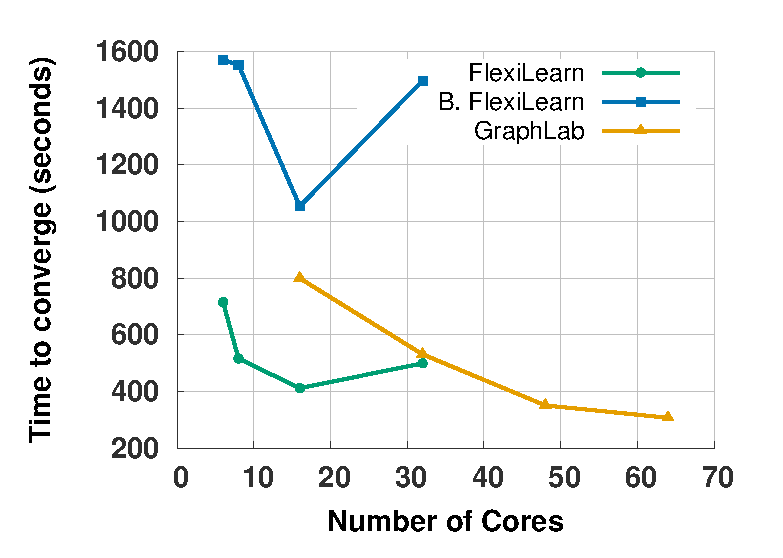
\includegraphics[width=0.23\textwidth]{fig2/lda_machines.eps} 
& 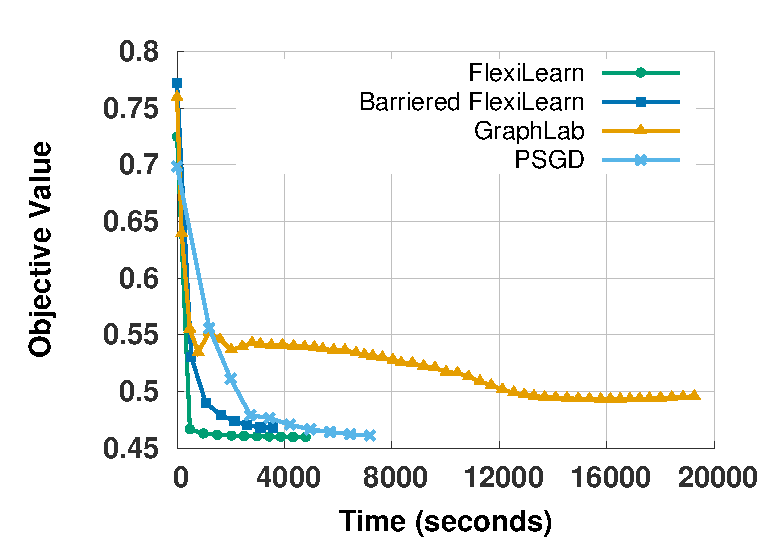
\includegraphics[width=0.23\textwidth]{fig2/dict_convergence.eps} 
& 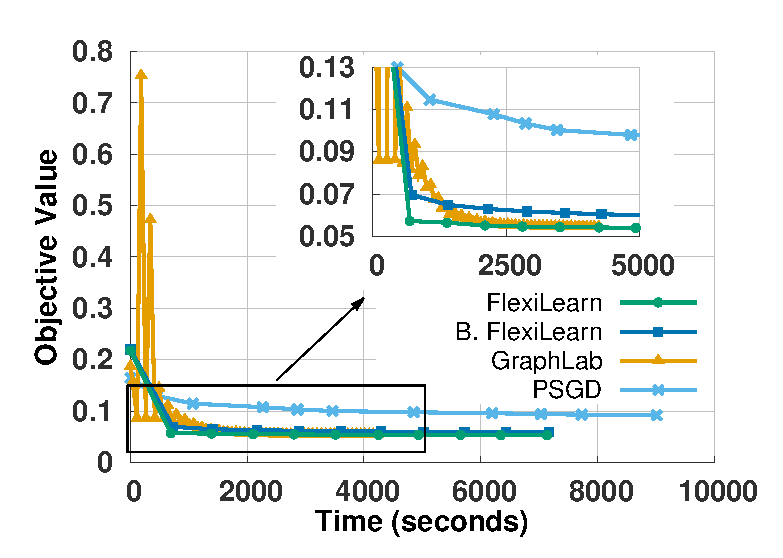
\includegraphics[width=0.23\textwidth]{fig2/mmsb_convergence.eps}  
\\
\hline
%{\bf Topic Modeling} & {\bf Dictionary Learning} & \multicolumn{2}{|c|}{\bf Mixed Membership Network Decomposition} \\
\multicolumn{4}{|c|}{\bf Topic Modeling} \\
\hline
Machines Needed & Scaling in \# Docs & \multicolumn{2}{|c|}{Scaling in \# Topics} \\
\hline
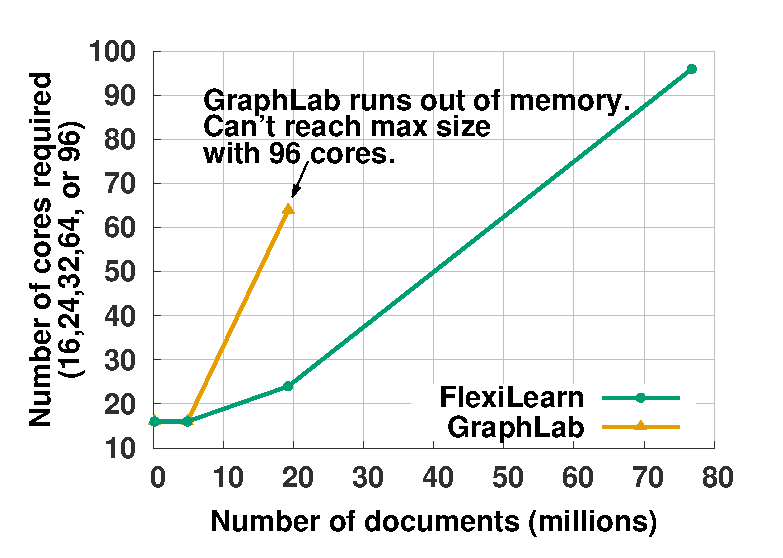
\includegraphics[width=0.23\textwidth]{fig2/lda_machines_failing.eps}
& 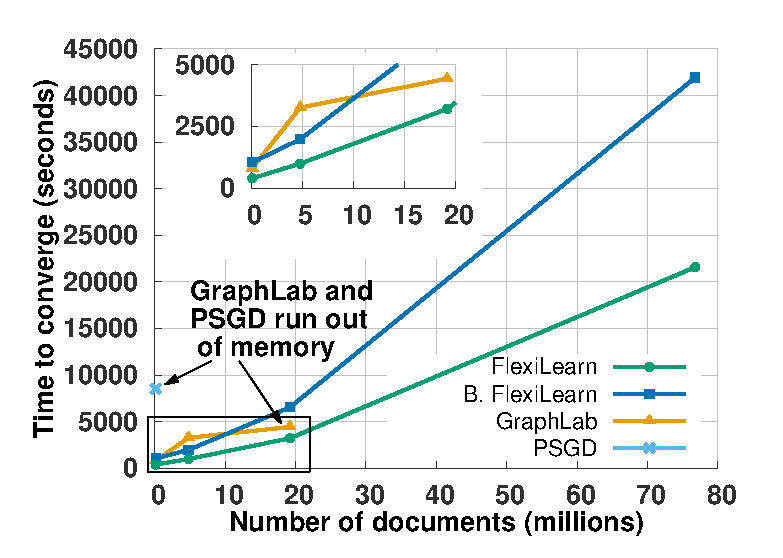
\includegraphics[width=0.23\textwidth]{fig2/lda_datasize.eps}
& \multicolumn{2}{|c|}{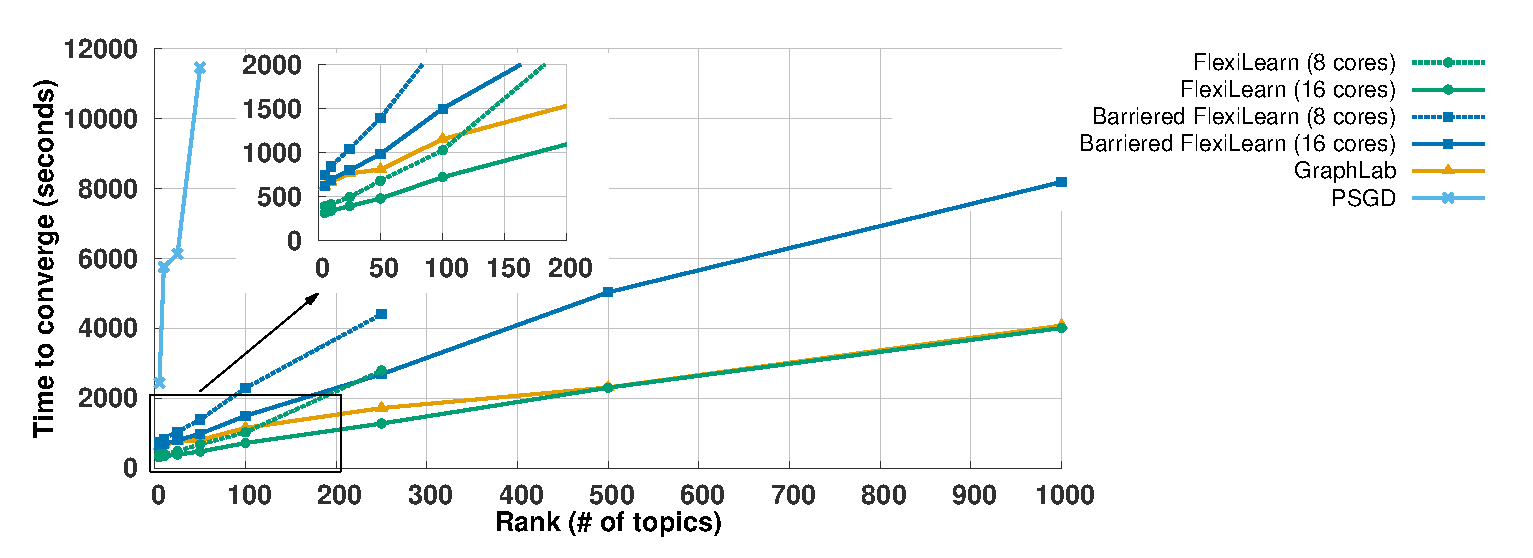
\includegraphics[width=0.46\textwidth]{fig2/lda_rankv2.eps}} \\
\hline
\end{tabular}
\vspace{-0.3cm}
\caption{\small Convergence and scalability plots for the three models (\lda, \dl, \mmsb),
under our \ourmethod{} and baselines (\dsgd, \psgd, \graphlab). Unless otherwise stated in the plot, all methods were run with 16 cores
and rank $K=25$. For all topic modeling plots except ``\# of Docs" and ``Machines Required", we used the NyTimes4 dataset (Table \ref{tab:dataset}).
The convergence plots reveal the objective trajectory and final value of each method,
while the scalability plots show how each method fares (on topic modeling) as we increase the problem rank, number of processor cores, and data size.
In the bottom left, we also show the minimum number of machines required for a given topic modeling dataset size, for
\ourmethod{} and \graphlab.}
\vspace{-0.5cm}
\label{fig:results}
\end{figure*}
\paragraph{Dataset size}
\begin{table}
\vspace{-0.2cm}
\centering
\scriptsize
\begin{tabular}{c|c|c|c|} %\hline
{\bf Dataset} & {\bf Dimensions} & {\bf Nonzeros} & {\bf Size (GB)} \\ \hline\hline
\nytimes  & $0.3*10^6\times$102,660 & $0.1*10^9$ &  1.49  \\ \hline
%\pubmed & $8.2*10^6\times$141,043 &  $0.73*10^9$ & 11.19  \\ \hline
\imagenet & $0.63*10^6\times$1,000 & $0.63*10^9$ & 7.99  \\ \hline
%\twitter & $41.6*10^6\times 41.6*10^6$ & $1.5*10^9$ & 23.99 \\ \hline
\webgraph & $0.28*10^6\times 0.28*10^6$ & $0.31*10^9$ & 4.46 \\ \hline
\snytimes{4} & $1.2*10^6\times$102,660 & $0.4*10^9$ &  6.08  \\ \hline
\snytimes{16} & $4.8*10^6\times$102,660 & $1.6*10^9$ &  25.12  \\ \hline
\snytimes{64} & $19.2*10^6\times$102,660 & $6.4*10^9$ &  103.4  \\ \hline
\snytimes{256} & $76.8*10^6\times$102,660 & $25.6*10^9$ &  421.42  \\
\hline
\end{tabular}
\vspace{-0.2cm}
\caption{\small Dimension, filesize and nonzero statistics for our datasets.
The biggest dataset (\snytimes{256}) is approximately 0.5
terabytes. Note that the \imagenet dataset is 100\% dense. }
\label{tab:dataset}
\vspace{-0.5cm}
\end{table}
data dimension
\paragraph{Model parameters}
rank
\paragraph{Processors}
machines, \method plateaus
\subsection{Convergence speed}
Figure~\ref{fig:speed} shows convergence times 
for \ourmethod{}, \dsgd, \psgd, and \graphlab over the three models: \lda, \mmsb and \dl. \ourmethod{} is faster
by anywhere between $2.6\times$ (vs \graphlab on \lda) to $26.2\times$ (vs \graphlab on \sdl).
\begin{figure}[t]
\vspace{-0.4cm}
\centering
\begin{tabular}{|c|c|}
\hline
 \multicolumn{2}{|c|} {\bf Time taken to converge} \\
\hline
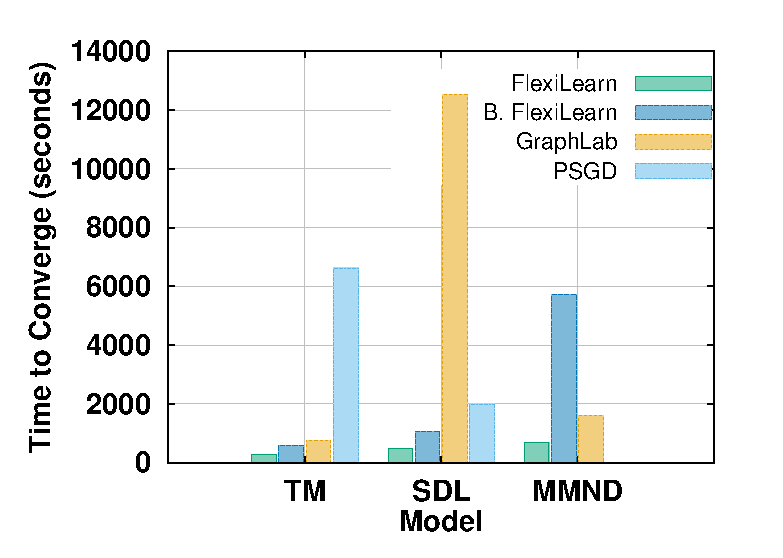
\includegraphics[width=0.46\columnwidth]{fig2/speedup.eps} &
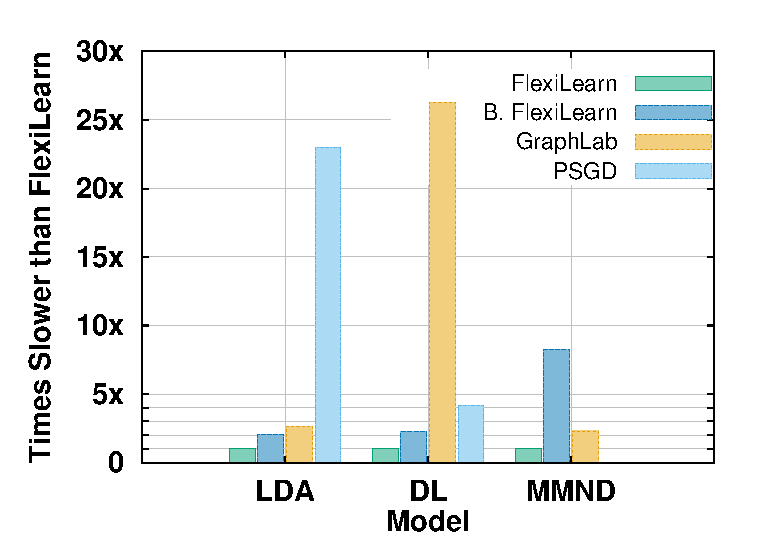
\includegraphics[width=0.46\columnwidth]{fig2/speedup2.eps} \\\hline
\end{tabular}
\vspace{-0.3cm}
\caption{\small Time taken by all methods to converge on the
three ML models, on an absolute scale (left) as well as a relative scale (right).
The methods plateau at these values in the respective plots shown
in figure~\ref{fig:results}. The bar for \psgd is absent in the figure as it never reaches $0.059$ and stops around 
objective value $0.092$.  }
\label{fig:speed}
\subsection{Convergence quality}
\graphlab oscillation reasons and patterns, \dsgd and \psgd converges to a poor
quality,
\subsection{Why \method wins }
Put a plot of waiting times in different concstraints case and argue why it
helps here.
